% This is samplepaper.tex, a sample chapter demonstrating the
% LLNCS macro package for Springer Computer Science proceedings;
% Version 2.20 of 2017/10/04
%
\documentclass[runningheads]{llncs}
%
\usepackage{graphicx}
\usepackage{enumitem}
\usepackage{amsmath,amssymb}
\usepackage{mathtext}

%\usepackage{hyperref}

\newcommand{\sign}{\operatorname{sign}}

%%%% ДЛЯ РУССКОГО ТЕКСТА закомментировать потом!
\usepackage{inputenc}
\usepackage[english,russian]{babel}
\usepackage{cmap}
%%%%


% If you use the hyperref package, please uncomment the following line
% to display URLs in blue roman font according to Springer's eBook style:
% \renewcommand\UrlFont{\color{blue}\rmfamily}

\begin{document}
%
\title{A search algorithm for the global extremum \break of a discontinuous function\thanks{This work was supported by the Russian Science Foundation, project No.\,21-11-00204.}}
%
\titlerunning{A search algorithm for the global extremum}
% If the paper title is too long for the running head, you can set 
% an abbreviated paper title here
%
\author{Konstantin Barkalov \orcidID{0000-0001-5273-2471}  
\and Marina Usova \orcidID{0000-0002-0722-6884}
}
%
\authorrunning{K. Barkalov, M. Usova}
% First names are abbreviated in the running head.
% If there are more than two authors, 'et al.' is used.
%
\institute{Lobachevsky State University of Nizhni Novgorod, Nizhni Novgorod, 
Russia \email{konstantin.barkalov@itmm.unn.ru}}
%
\maketitle              % typeset the header of the contribution
%
\begin{abstract}
We consider the problem of finding the global minimum of a one-dimensional function that may have several finite jump discontinuity points. The discontinuities of the objective function can reflect the specifics of the optimized object in the mathematical model (for example, shock effects, resonance phenomena, jumps in geometric dimensions or material properties, etc.). In some cases, the discontinuing set is known. However, at the same time, there are problems in which there are no a priori estimates of discontinuity points, but it is known that such points are possible. The paper gives a description of the global search algorithm for solving the specified class of problems. The authors conducted an experimental comparison of the proposed algorithm with the methods implemented in MATLAB Global Optimization Toolbox.

\keywords{Global optimization \and Multiextremal functions \and Discontinuous functions \and Algorithms' comparison }

\end{abstract}
%
%
%
\section{Introduction}

This paper considers the problem of finding the global minimum $x^*$ of a one-dimensional function $\varphi(x)$ of the form 
\begin{equation}\label{problem}
\varphi(x^*)=\min\left\{\varphi(x):x\in\left[a,b\right]\right\}.
\end{equation}

Global optimization problems involving many local extrema arise in many areas of applications (see, e.g., \cite{Cavoretto2021,Kvasov2013,Kvasov2015,Modorskii2016}). As a rule, the calculation of even a single value of the objective function in such problems requires considerable time, since the analytical form of the function is not known and the calculation of its values involves time-consuming numerical modelling. In this case, we have to deal with expensive black-box optimization problems as they are often called. Problems of this class are extremely complicated and are the object of intensive research.

One should note an important role of one-dimensional global optimization problems. Firstly, as has already been mentioned, they arise in many applications (see, e.g., \cite{Gillard2017,Sergeyev2020}). Secondly, many approaches to solving multidimensional optimization problems are, in one way or another, based on reducing the solution of the original multidimensional problem to solving a series of related one-dimensional optimization problems (see, for example, popular approaches in \cite{PaulaviciusZilinskas2014,Pinter1996,Sergeyev2017,Sergeyev2013}).

The literature describes various methods for solving the problem (\ref{problem}) depending on the assumptions about the properties of the objective function \cite{Horst1995,Horst1996,Pinter1996}. One of such assumptions, which is often fulfilled in applied optimization problems, is that the objective function $\varphi(x)$ satisfies the Lipschitz condition 
\[
\left|\varphi(x')-\varphi(x'')\right|\leq L\left|x'-x''\right|,\; x',x'' \in [a,b],
\]
where the constant $L$ is unknown a priori. 
This feature of the objective function is commonly used in many approaches to the development of algorithms for multiextremal optimization \cite{Evtushenko2009,Evtushenko2013,Jones2009,Paulavicius2011}.



However, in some applied problems, the Lipschitz property may not be fulfilled due to the presence of discontinuous jumps in the values of the function at some points of the search domain. Such jumps can be caused by sharp changes in the characteristics of the optimized object with small changes in its parameters, for example:
\begin{itemize}
  \item changes in the thickness of the material (or other geometric parameters of the object);
  \item changes in material properties (both when different materials are used in one design, and with changes in the properties of the same material as a result of technological operations, for example, welding, etc.);
  \item changes in external sources of impact (temperature, force, etc.).
\end{itemize}

We will interpret such sharp changes as jump discontinuities. For these cases, the set of points, at which the characteristics of the object jump, is typically known in advance. However, at the same time, there are problems in which there are no a priori estimates of discontinuity points, but it is known that such points are possible.

The known methods for solving such problems, as a rule, either generalize the concept of a gradient for discontinuous functions \cite{Batukhtin1993,Batukhtin1998,Moreau2000}, or belong to the class of bio-inspired algorithms \cite{Ban2019,ZhangXu}. These methods provide, generally speaking, the search for only a local solution to the problem.

In this paper, we will consider a deterministic algorithm for solving global optimization problems with both given and unspecified discontinuity points. This algorithm was developed on the basis of the \textit{global search algorithm} proposed by Strongin \cite{Strongin2000} and provides a search for the global optimum. Section 2 describes the algorithm for functions with given discontinuities. Section 3 discusses how to identify unspecified discontinuities. Section 4 describes how this discontinuity detection method can be used in the original algorithm. Section 5 presents the results of a comparison of the developed algorithm with the global search methods implemented in MATLAB Global Optimization Toolbox \cite{MatlabOTB}. Section~6 concludes the paper. 

\section{Algorithm for functions with given discontinuity points}

Let us consider problem (\ref{problem}) assuming that the objective function $\varphi(x), x\in[a,b],$ has jump discontinuities at the given points
\begin{equation}\label{points}
a = \omega_0 <\omega_1 < ... <\omega_s < \omega_{s+1} = b
\end{equation}
and satisfies the Lipschitz condition between them, i.e.
\begin{equation}\label{LipschitzСondition}
\left|\varphi(x')-\varphi(x'')\right|\leq L\left|x'-x''\right|, \; x',x'' \in (\omega_{i-1},\omega_{i}), \; 1 \leq i \leq s+1.
\end{equation}
Points $\omega_{0}$ and $\omega_{s+1}$ are included in the general list regardless of the presence of function discontinuities in them for the convenience of subsequent presentation. Let us denote the resulting set of points $\Omega$, i.e. $\Omega = \{\omega_{0}, ..., \omega_{s+1}\}$, where $\omega_{0} = a, \; \omega_{s+1} = b$.

In \cite{Strongin2000}, the global search algorithm (GSA) was considered for solving problems without discontinuities. The authors also proposed a method for accounting for discontinuities based on a smoothing transformation of the objective function. Below we consider an algorithm based on GSA, in which the discontinuous function is minimized without smoothing of the discontinuities, which greatly simplifies the computational scheme of the algorithm.

In the preliminary step of the method, the first $s+1$ trials are carried out at arbitrary interior points $x^i \in (\omega_{i-1},\omega_{i}), \; 1 \leq i \leq s+1 $. A point $x^{k+1}$, $k \geq s+1$, for the next trial is selected as follows.

\begin{enumerate}
\item Arrange prior trial points $x^1,...,x^k$ and points $\omega_{0}, ..., \omega_{s+1}$ in ascending coordinate order. Designate the points of the resulting single series $x_i, 0\leq i \leq m = k + s + 1$,
\begin{equation}\label{pointsX}
a = x_0 < x_1 < ... < x_{m-1} < x_{m} = b,
\end{equation}
and match them with values $z_i=\varphi(x_i)$ for $x_i \not\in \Omega$. Note that, in accordance with the choice of trial points at the preliminary step of the algorithm, there will be no interval $(x_{i-1},x_i)$, the boundary points of which simultaneously belong to the set $\Omega$.

\item For each interval $(x_{i-1},x_i ), 1\leq i \leq m$, calculate the values
\begin{equation}\label{mu_i}
\mu_i=(1-\gamma_i-\gamma_{i-1} )  \frac{|z_i-z_{i-1} |}{(x_i-x_{i-1} )}
\end{equation}
where
\begin{equation}\label{gamma}
\gamma_i = 
\begin{cases}
	1, &\text{$x_i \in \{\omega_{0},...,\omega_{s+1}\} $}, \\
	0, &\text{$x_i \not\in \{\omega_{0},...,\omega_{s+1}\}. $}
\end{cases}
\end{equation}
Find the maximum value 
%\begin{equation}\label{mu}
\[
\mu=\max\left\{\mu_i: 1 \leq i \leq m\right\}.
\]
%\end{equation}
When $\mu=0$, use the value $\mu=1$.
Note that rule (\ref{gamma}) ensures that the inequality $0 \leq \gamma_i+\gamma_{i-1} \leq 1$ holds for every $1 \leq i \leq m$. Therefore, the value $\mu_i$ will be equal to 0 if one of the endpoints of the interval $ (x_{i-1},x_i ), \; 1 \leq i \leq m,$ belongs to $\Omega$.

\item For each interval $(x_{i-1},x_i), \; 1\leq i \leq m,$ calculate the characteristic
\begin{equation}\label{R_i}
\begin{gathered}
R(i)=(1+\gamma_i+\gamma_{i-1} )\Delta_i+(1-\gamma_i-\gamma_{i-1} ) \frac{ (z_i-z_{i-1} )^2}{(r\mu)^2 \Delta_i }-\\
-\frac{2[(1-\gamma_i )(1+\gamma_{i-1} ) z_i+(1+\gamma_i )(1-\gamma_{i-1} ) z_{i-1} ]}{r\mu},
\end{gathered}
\end{equation}
where $r>1$ is the method parameter.

\item Determine the interval to which the maximum characteristic corresponds 
%\begin{equation}\label{R_max}
\[
R(t)=\max\left\{R(i): 1 \leq i \leq m\right\}.
%\end{equation}
\]

\item Carry out next trial at the point
%\begin{equation}\label{new_x}
\[
x^{k+1}=\frac {(x_t+x_{t-1})}{2}-(1-\gamma_t-\gamma_{t-1} ) \frac{(z_t-z_{t-1})}{2r\mu}.
%\end{equation}
\]

\item Check termination condition $x_t-x_{t-1} \leq \epsilon$, where $t$ is the number of the interval with the maximal characteristic and $\epsilon > 0$ is the predefined accuracy.

\end{enumerate}

%Russian
\textbf{Remark 1}. Еще раз отметим, что в соответствии с (\ref{gamma}) значение $\gamma_i+\gamma_{i-1}$ может быть равно либо 0 (обе граничных точки интервала принадлежат области непрерывности функции), либо 1 (одна из граничных точек является точкой разрыва). В этом случае формула (\ref{R_i}) иметь вид
\[
R(i)=\Delta_i+\frac{ (z_i-z_{i-1} )^2}{(r\mu)^2 \Delta_i }-\frac{2(z_i + z_{i-1})}{r\mu},
\]
в случае отстутсвия точке разрыва и 
\[
R(i)=2\Delta_i - \frac{4 z_i }{r\mu}, \; R(i)=2\Delta_i - \frac{4 z_{i-1} }{r\mu},
\]
в случае разрыва в точке $x_{i-1}$ или $x_{i}$ соответственно.

\textbf{Remark 2}.
Приведенные выше формулы для вычисления характеристик интервалов могут быть использованы (в модифицированной форме) в алгоритме решения задач невыпуклыми ограничениями \cite{Sergeyev1995,Sergeyev2006_1,Sergeyev2007}. Здесь решение задачи с частично определенными ограничениями неявно сводится к минимизации разрывной функции, в которой точками разрыва являются границы допустимого множества решений задачи.


\textbf{Remark 3}. The erroneous assignment of some discontinuity points from the series (\ref{points}) will not lead to the loss of convergence of the method. The algorithm will interpret such points as a recoverable discontinuity case since the left and right limits of the objective function at such points coincide.

It can be proved that the conditions for the convergence of this algorithm will correspond to the conditions for the convergence of its basic prototype -- the global search algorithm from \cite{Strongin2000}. The formulation and rigorous proof of the convergence conditions will be the subject of further publications.

Let us illustrate the operation of the algorithm when searching for the minimum of the function
\begin{equation}\label{testFunction}
\varphi(x) =  0.1\sum_{i=1}^5{i\sin{(10(i+1)x+i)}}+
\begin{cases}
	-4, &0 \leq x < 3.1\\
	10, &3.1 \leq x < 4.6\\
	0, &4.6 \leq x < 7.0\\
	30, &7.0 \leq x < 9.0\\
	0, &9.0 \leq x \leq 10.0
\end{cases}
\end{equation}
at $x\in[0,10]$. All discontinuity points were considered known, the parameters of the method $r=2.0,\epsilon=0.001$ were used. Fig.~\ref{ris1} shows a graph of this function, the discontinuities are marked with a dotted line. The dashes under the graph indicate the points of 70 trials required for the algorithm to solve problem with the specified accuracy.

\begin{figure}[ht]
	\begin{center}
			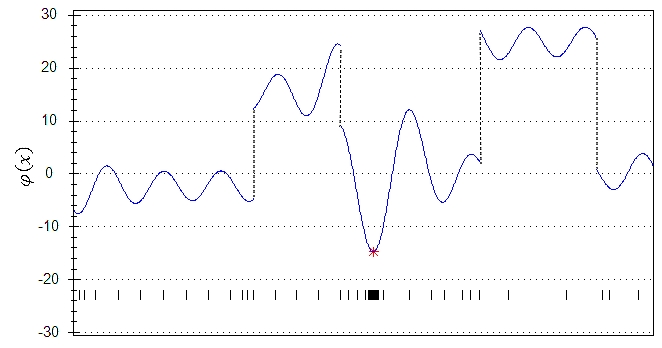
\includegraphics[width=0.9\linewidth]{ris_1.jpg}
			\caption{Discontinuous objective function graph and trial points in case of given discontinuity points}
      \label{ris1}
	\end{center}
\end{figure}

\section{Identifying Unspecified Discontinuities}

Let us suppose now that the location of the discontinuity points for the function $\varphi(x)$ is not known, but it is known that such points are possible. Let the function have a discontinuity at an a priori unknown point $\omega \in(x_{i-1},x_i)$, then the relative difference $\mu_i$ from (\ref{mu_i}) will significantly exceed the relative differences for other intervals since within them the function satisfies the Lipschitz condition. Therefore, the identification of such situations can be based on a comparison of the relative differences $\mu_i$ from (\ref{mu_i}) corresponding to different search intervals $(x_{i-1},x_i)$.

Let us enumerate the differences $\mu_i$ from (\ref{mu_i}) in decreasing order (by the index in brackets)

\begin{equation}\label{mu_cond}
\mu(1) \geq \mu(2) \geq ... \geq \mu(m)
\end{equation}
and define the minimum number $p$ satisfying the conditions
\begin{equation}\label{mu_main_cond}
 \frac{\mu(p)}{\mu(p+1)} \geq Q, \; 1 \leq p < q(m-2(s+1)),
\end{equation}
where $Q>1$ and $0<q<1$ are parameters.
%Russian
Значение параметра $Q$ определяет наши априорные предположения о том, во сколько раз относительная разность $\mu_i$, вычисленная на интервале $(x_{i-1},x_i)$, содержащем точку разрыва, будет превышать максимальную разность $\mu$, найденную по всем интервалам, принадлежащим области непрерывности функции. Данное значение задается исследователем, и в проведенных эксмериментах оно было выбрано равным 3.


When at the current $k$-th iteration of the method there is no $p$ that satisfies these conditions, it is interpreted as the absence of unspecified discontinuities. If such $p$ exists, this situation corresponds to the presence of undefined discontinuities. In this case, zero differences $\mu_i$ from (\ref{mu_i}), corresponding to intervals containing specified discontinuity points, are excluded from consideration by the condition $p<m-2(s+1)$.

Note that the value of the difference $\mu_i$ for the interval containing the extremum point can be close to zero, which will lead to the fulfillment of the first inequality from (\ref{mu_main_cond}). To eliminate the effect of small relative differences of intervals containing extreme points, the additional constraint $1 \leq p < q(m-2(s+1))$ is introduced in (\ref{mu_main_cond}) to exclude small values of $\mu_i$ from consideration. 
%Russian
Значение параметра $q$ отражает априорные предполжения о том, какая доля поисковых интервалов в их общем числе не будет содержать точек локальных экстремумов. 


Let us select a subset of numbers
\begin{equation}\label{set_I}
I=\left\{ i:1 \leq i \leq m, \; \mu_i=\mu(j), \; 1 \leq j \leq p\right\}
\end{equation}
of the intervals $(x_{i-1},x_i)$, which correspond to large relative differences $\mu_i$. Large difference values are interpreted as the presence of undefined discontinuities in the intervals $(x_{i-1},x_i), i \in I$. Moreover, the set $I$ can change in the process of solving the problem.

\section{Algorithm for unspecified discontinuities}

The algorithm is a modification of the algorithm described in Section 2 for given discontinuities and consists of the following. 

The first $s+1$ trials are carried out at arbitrary interior points $x^i \in (\omega_{i-1},\omega_i )$,  $1 \leq i \leq s+1$, where the set $\Omega=\{\omega_0,...,\omega_{s+1}\}$ contains the given discontinuity points, as well as boundary points $\omega_0=a$ and $\omega_{s+1}=b$. A point for the next trial $x^{k+1}, \; k \geq s+1$, is selected as follows.

\begin{enumerate}
\item Sort points of a set $\{x^1,...,x^k\} \cup \Omega$ in ascending order of coordinates 
\begin{equation}\label{x_cond}
 a=x_0<x_1<...<x_{m-1}<x_m=b,
\end{equation}
where $m=s+k+1$. Each point is matched with an attribute $\gamma_i$ from (\ref{gamma}) (the presence or absence of a set discontinuity) and with the value of the function $z_i=\varphi(x_i)$ calculated only for $x_i \not\in \Omega$, i.e. at $\gamma_i=0$.

\item Calculate the relative differences $\mu_i, \; 1 \leq i \leq m$, from (\ref{mu_i}) and order them in descending order, i.e. build a series (\ref{mu_cond}).

\item Determine $p$ satisfying the inequalities (\ref{mu_main_cond}), where $0<q<1<Q$ are the parameters of the algorithm. Construct a set $I$ from (\ref{set_I}), the elements of which are interpreted as numbers of intervals that can contain a discontinuity. Generate interval attributes
\begin{equation}\label{delta_cond}
\delta_i=
\begin{cases}
	\sign{(z_i - z_{i-1})}, &\text{$i \in I$}, \\
	0, &\text{$i \not \in I$}.
\end{cases}
\end{equation}
The value $\delta_i=-1$ corresponds to a sharp decrease in the function in the interval $(x_{i-1},x_i)$, $\delta_i=1$ -- to an increase, $\delta_i=0$ -- to the lack of jump. Note that in accordance with the rules (\ref{gamma}) and (\ref{delta_cond}) for calculating attributes $\gamma_i$ and $\delta_i$ the inequalities
$ 0 \leq \gamma_i+\gamma_{i-1}+|\delta_i | \leq 1, \; 1 \leq i \leq m, $
are met.

\item Determine the maximum value
\begin{equation}\label{mu_new}
\mu=\max\left\{\left(1-\gamma_i-\gamma_{i-1}-|\delta_i|\right) \frac {|z_i-z_{i-1}|}{(x_i-x_{i-1})}: 1 \leq i \leq m\right\}.
\end{equation}
When $\mu=0$, use the value $\mu=1$.

\item For each interval $(x_{i-1},x_i), \; 1 \leq i \leq m$, calculate the characteristic
%\begin{equation}\label{R_new}
\[
\begin{gathered}
R(i)=(1+\gamma_i+\gamma_{i-1}+|\delta_i |) \Delta_i+(1-\gamma_i-\gamma_{i-1}-|\delta_i |)\frac{(z_i-z_{i-1} )^2}{(r\mu)^2 \Delta_i } - \\
- \frac{2[((1-\gamma_i )(1+\gamma_{i-1} )(1-\delta_i )) z_i+((1+\gamma_i )(1-\gamma_{i-1} )(1+\delta_i )) z_{i-1} ]}{r\mu},
\end{gathered}
%\end{equation}
\]
where $r > 1$ is the method parameter, $\mu$ is from (\ref{mu_new}) and $\Delta_i=x_i-x_{i-1}$.

\item Determine the interval corresponding to the maximum characteristic
%\begin{equation}\label{R}
\[
R(t)=\max\left\{R(i): 1 \leq i \leq m\right\}.
\]
%\end{equation}

\item Carry out next trial at the point 
\begin{equation}\label{new_x_2}
x^{k+1}=\frac {(x_t+x_{t-1})}{2}-(1-\gamma_t-\gamma_{t-1}- |\delta_t|) \frac{(z_t-z_{t-1})}{2r\mu}.
\end{equation}

\item Check the termination condition $x_t-x_{t-1} \leq \epsilon$, where $t$ is the number of the interval with the maximal characteristic and $\epsilon > 0$ is the predefined accuracy.
\end{enumerate}

%Russian
\textbf{Remark}. В соответствии с (\ref{gamma}) and (\ref{delta_cond}) значение $\gamma_i+\gamma_{i-1}+|\delta_i |$ может быть равно 0 либо 1, в зависимости от наличия либо отсутствия точки разрыва в интервале $(x_{i-1},x_i)$.
Так, если данный интервал не содержит точек разрыва, т.е. $\gamma_i+\gamma_{i-1}+|\delta_i | = 0$, его характеристика (\ref{R_i}) пример вид 
\[
R(i)=\Delta_i+\frac{ (z_i-z_{i-1} )^2}{(r\mu)^2 \Delta_i }-\frac{2(z_i + z_{i-1})}{r\mu}.
\]
Если одна из граничных точек интервала является заданной точкой разрыва, т.е. $\gamma_{i-1} = 1$ или $\gamma_i = 1$, то мы получим соответственно характеристики
\begin{equation}\label{RR}
R(i)=2\Delta_i - \frac{4 z_i }{r\mu}, \; R(i)=2\Delta_i - \frac{4 z_{i-1} }{r\mu}.
\end{equation}
Аналогичные формулы для характеристик интервалов будут получаться, если $(x_{i-1},x_i)$ является интервалом, который содержит незаданную точку разрыва, т.е. когда $|\delta_i | = 1 $. В этом случае мы таже будем получать формулы (\ref{RR}) для $\delta_i = -1$ и $\delta_i = 1$, что соответствует использованю результатов испытания в правой точке интервала для построения его характеристики в случае убывания функции и выбору левой точки при возрастании функции.


Fig.~\ref{ris2} shows the results of solving the problem from the previous example (\ref{testFunction}), in which the discontinuity points were considered unspecified. Here we used the parameters of the method $r=2.0, \epsilon=0.001, Q=3.0, q=0.3$. The dashes under the graph indicate the points of 70 trials required for the algorithm to solve problems with the specified accuracy.

\begin{figure}%[!ht]
	\begin{center}
			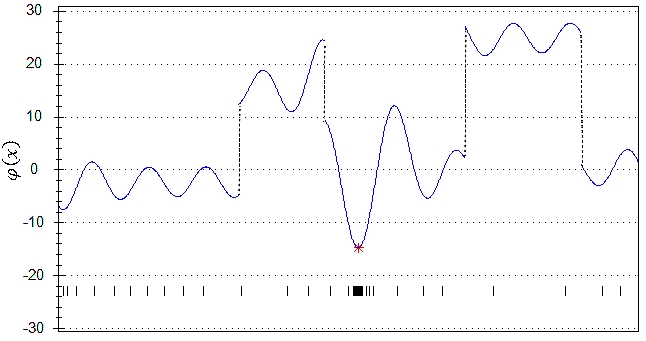
\includegraphics[width=0.9\linewidth]{ris_2.jpg}
			\caption{Discontinuous objective function graph and trial points in case of unspecified discontinuity points}
      \label{ris2}
	\end{center}
\end{figure}

\begin{figure}%[!ht]
	\begin{center}
			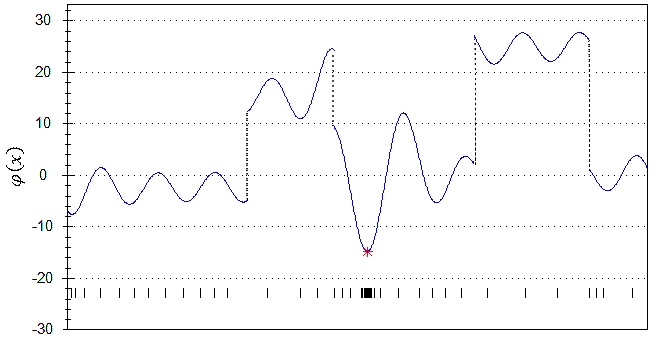
\includegraphics[width=0.9\linewidth]{ris_3.jpg}
			\caption{Discontinuous objective function graph and trial points in case of partially given discontinuity points}
      \label{ris3}
	\end{center}
\end{figure}

The proposed algorithm also allows partial specification of known discontinuities. Fig.~\ref{ris3} shows the results of solving the same problem, for which the discontinuities were considered partially given (the discontinuities at the points 4.6 and 9.0 were considered to be known). Here we used the same parameters of the method $r=2.0, \epsilon=0.001, Q=3.0, q=0.3$. The dashes under the graph indicate the points of 67 trials required for the algorithm to solve problems with the specified accuracy.

\section{Results of Numerical Experiments}

To demonstrate the efficiency of the global search algorithm for discontinuous functions (GSA-D) described in the previous section, we compare it with Direct Search (DS) \cite{Audet}, Simulated Annealing (SA) \cite{Kirkpatrick}, and Genetic Algorithm (GA) \cite{Goldberg} implemented in MATLAB Global Optimization Toolbox \cite{MatlabOTB}.

As the main comparison criterion, we will use the number of search trials $K$ (i.e., the number of calculations of the objective function) performed by the method before it converges.

The algorithms were compared when solving 1000 problems with a discontinuous objective function, which were constructed as follows. First, we generated continuous functions of the form
\begin{equation}\label{seriaFunction}
f(x) =  \sum_{j=0}^4{(j+1)A_j\sin{(5\pi jx+j)}+(j+1)B_j\cos(3\pi jx+j)}, x\in[0,1],
\end{equation}
where the values of the coefficients $A_j, B_j$ were chosen randomly and uniformly from the interval $[-6,6]$. Then 4 discontinuity points were added to the continuous functions. The coordinates of these points $\omega_1, \; \omega_2, \; \omega_3, \; \omega_4$ were set randomly and uniformly from the ranges $[0,0.25), \; [0.25,0.5), \; [0.5,0.75), \; [0.75,1]$ respectively. The jump values $\delta_1, \; \delta_2, \; \delta_3, \; \delta_4$ at discontinuities were also randomly selected from the range $[-50,50]$. These operations produced a discontinuous function of the form
\begin{equation}\label{seriaFunction_jump}
\varphi(x) =  f(x)+
\begin{cases}
	\delta_1, &0 \leq x < \omega_1\\
	\delta_2, &\omega_1 \leq x < \omega_2\\
	\delta_3, &\omega_2 \leq x < \omega_3 \;, \;\;\; x\in[0,1].\\
	\delta_4, &\omega_3 \leq x < \omega_4\\
	\delta_1, &\omega_4 \leq x \leq 1.0
\end{cases}
\end{equation}

Since the solution of the test problem assumes that the global optimizer $x^*$ is known, its value was preemptively estimated for each function of the series by iterating through all nodes of a uniform grid, the step of which was chosen to be sufficiently small.

The first experiment was performed when solving a series of 1000 problems with continuous functions of the form (\ref{seriaFunction}). Table~\ref{tab1} shows the number of problems solved, the average number of iterations performed by different methods for solving the series, and the number of trials performed by the methods during the search. The problem was considered solved if the condition $|x^k-x^* | \leq \delta$ was met for the trial point $x^k$, where $x^*$ is the known solution of the problem and $\delta= 10^{-2}$. At the same time, the accuracy used in the termination criteria for all methods was $\epsilon = 10^{-3}$.

In order to exclude the influence of inherent randomness when running algorithms from MatLab, the GA, SA, and DS methods were run 5 times for each problem, and the best result was recorded (in terms of the proximity of the found solution to the true one). In this case, the GA and SA methods were run with default parameters, while in the DS method the parameter $x_0$ (the starting point of the search) varied from 0 to 1 with a step of 0.2.

With multiple runs, the methods from MATLAB Global Optimization Toolbox solved almost all the problems in the series, while with a single run of these methods the number of correctly solved problems was almost 2 times less. At the same time, the GSA-D method successfully solved all the problems in the series (the reliability parameter $r=2.2$ was used for the method). At the same time, the number of trials spent was comparable to the DS method and significantly less than the number of trials of the GA and SA methods.

\begin{table}[ht]
	\caption{Results of solving a series of problems with continuous functions}
	\label{tab1}
	\begin{center}
		\begin{tabular}{c|c|c|c}
			\hline
			Method & Problems solved & Average number of iterations & Average number of trials \\
			\hline
%			\hline
                                GSA-D & 1000  &  52  &  53 \\
                                \hline
                                SA    &  1000  &  774  &  777  \\
			\hline
			GA    &   999  &  24  &  1290  \\
			\hline
                                DS    &  970  & 38  &  71  \\
			\hline
		\end{tabular}
	\end{center}
\end{table}

The next experiment was performed when solving a series of 1000 problems with discontinuous functions of the form (\ref{seriaFunction_jump}).  GSA-D used the parameters $r=3.7, \; Q=3.0, \; q=0.3$, the other experimental conditions were similar to the previous run. The results of solving a series of problems with discontinuous functions are shown in Table~\ref{tab2}.

\begin{table}[ht]
	\caption{Results of solving a series of problems with discontinuous functions}
	\label{tab2}
	\begin{center}
		\begin{tabular}{c|c|c|c}
			\hline
			Method & Problems solved & Average number of iterations & Average number of trials \\
			\hline
%			\hline
                                GSA-D & 1000  & 79  &  80 \\
                                \hline
                                SA    &  998  &  765  &  770  \\
			\hline
			GA    &   993  &  25  &  1310  \\
			\hline
                                DS    &  964  & 38  &  71  \\
			\hline
		\end{tabular}
	\end{center}
\end{table}

The results show that the Global Optimization Toolbox methods solve discontinuous problems somewhat worse than continuous ones, while the GSA-D algorithm proposed in the paper successfully solves the entire series of problems. The GA and SA algorithms show high reliability of finding the global optimizer after several runs, but these methods significantly lose to the GSA-D algorithm in terms of the number of objective function calculations. The DS method, showing a comparable number of trials, is inferior in the number of correctly solved problems.

Summing up, we note that although the methods from the MATLAB Global Optimization Toolbox are stated as methods that work with discontinuous functions, they do not guarantee convergence to the global minimum. The convergence rate (in terms of the number of trials) for the GA and SA methods is significantly lower than that for the DS method. However, the DS algorithm, while surpassing the GA and SA methods in this indicator, has the lowest reliability among the considered methods. The GSA-D method proposed in the article demonstrated both the guaranteed convergence to the global minimizer for the problems with discontinuous functions and the smaller number of trials required to achieve convergence.

\section{Conclusion}

In this paper, we propose an algorithm for finding the minimum of a multiextremal function with jump discontinuities. The proposed GSA-D algorithm, unlike many known approaches, does not use the concept of a gradient and provides a search for a global solution to the problem. We carried out computational experiments confirming the convergence of the algorithm for a wide class of discontinuous multiextremal problems. The convergence conditions of the proposed algorithm, in general, will correspond to the convergence conditions of its prototype -- the global search algorithm for continuous problems, considered in detail in \cite{Strongin2000}. Justification and research of the theoretical properties of the proposed GSA-D algorithm will be the subject of future publications.


%
% ---- Bibliography ----
%
% BibTeX users should specify bibliography style 'splncs04'.
% References will then be sorted and formatted in the correct style.
%
 \bibliographystyle{splncs04}
 \bibliography{bibliography}


\end{document}
